\subsection{Đề 5}
\Opensolutionfile{ans}[ans/ans-2-B1-De1-LC]
\caulc
\begin{ex}%[Câu 1]%[1D1N4-5]
	Trong các hàm số sau hàm số nào tuần hoàn với chu kỳ $2\pi $.
	\choice
	{$y= \cos 2x$}
	{\True $y= \sin x$}
	{$y= \tan 2x$}
	{$y= \cot 2x$}
	\loigiai{
	Hàm số $y=\sin x$ tuần hoàn với chu kì $2 \pi$.
	}
\end{ex}

\begin{ex}%[Câu 2]%[1D1N1-2]
	Nếu một cung tròn có số đo là $20$ độ thì số đo radian của nó là 
	\choice
	{$\dfrac{\pi}{10}$}
	{\True $\dfrac{\pi}{9}$}
	{$\dfrac{\pi}{8}$}
	{$\dfrac{\pi}{11}$}
	\loigiai{
		Sử dụng công thức: $\alpha^\circ=\alpha \cdot \dfrac{\pi}{180} \mathrm{rad}$. Ta có: $20^\circ=20 \cdot \dfrac{\pi}{180}=\dfrac{\pi}{9}$.
	}
\end{ex}

\begin{ex}%[Câu 3]%[1D1N3-2]
	Chọn đáp án đúng
		\choice 
		{\True $\sin a-\sin b=2 \cos \dfrac{a+b}{2} \sin \dfrac{a-b}{2}$}
		{$\sin a-\sin b=\cos \dfrac{a+b}{2} \sin \dfrac{a-b}{2}$}
		{$\sin a-\sin b=2 \sin \dfrac{a+b}{2} \cos \dfrac{a-b}{2}$}
		{$\sin a-\sin b=\sin \dfrac{a+b}{2} \cos \dfrac{a-b}{2}$}
	\loigiai{
		Công thức $\sin a-\sin b=2 \cos \dfrac{a+b}{2} \sin \dfrac{a-b}{2}$.
	}
\end{ex}

\begin{ex}%[Câu 4]%[1D1H1-1]
	Xét góc lượng giác $(OA,OM)=\alpha$, trong đó $M$ là điểm không nằm trên các trục tọa độ $Ox$ và $Oy$. Khi đó, $M$ thuộc góc phần tư nào để giá trị $\sin \alpha$ và $\cos \alpha$ trái dấu?
	\choice
	{Góc phần tư thứ $(\text{I})$ và $(\text{II})$}
	{Góc phần tư thứ $(\text{I})$ và $(\text{III})$}
	{\True Góc phần tư thứ $(\text{II})$ và $(\text{IV})$}
	{Góc phần tư thứ $(\text{II})$ và $(\text{III})$}
	\loigiai{
		Ta có:\\
		Với $\alpha \in$ góc phần tư thứ $\text{I}$ thì: $\sin \alpha>0, \cos \alpha>0$.\\
		Với $\alpha \in$ góc phần tư thứ $\text{II}$ thì: $\sin \alpha>0, \cos \alpha<0$.\\
		Với $\alpha \in$ góc phần tư thứ $\text{III}$ thì: $\sin \alpha<0, \cos \alpha<0$.\\
		Với $\alpha \in$ góc phần tư thứ $\text{IV}$ thì: $\sin \alpha<0, \cos \alpha>0$.\\
		Do đó, $M$ thuộc góc phần tư thứ $\text{II}$ và $\text{IV}$ thì $\sin \alpha$ và $\cos \alpha$ trái dấu.
	}
\end{ex}

\begin{ex}%[Câu 5]%[1D2H3-1]
	Cho cấp số nhân $(u_n)$ có số hạng đầu $u_1$ và công bội $q$. Số hạng tổng quát $u_n$ được xác định theo công thức:
	\choice
	{$u_n=u_1+(n-1)q$ với $n \ge 2$}
	{$u_n=u_1+nq$ với $n \ge 2$}
	{$u_n=u_1 \cdot q^n$ với $n \ge 2$}
	{\True $u_n=u_1 \cdot q^{n-1}$ với $n \ge 2$}
	\loigiai{ 
		Cấp số nhân $(u_n)$ có số hạng đầu $u_1$ và công bội $q$. Số hạng tổng quát $(u_n)$ được xác định theo công thức: $u_n=u_1 \cdot q^{n-1}$ với $n \ge 2$.
	}
\end{ex}

\begin{ex}%[Câu 6]%[1D2H1-5]
	Cho dãy số $(u_n)$ với $u_n=25n^2+10n+9$. Chọn khẳng định đúng
	\choice
	{\True Dãy số trên bị chặn dưới}
	{Dãy số trên bị chặn trên}
	{Dãy số trên không bị chặn}
	{Dãy số trên bị chặn}
	\loigiai{
		Ta có: $u_n=25 n^2+10 n+9=\left(25 n^2+10 n+1\right)+8=(5 n+1)^2+8 \geq 8$ với mọi $n \in \mathbb{N}^*$.\\
		Do đó, dãy số $\left(u_n\right)$ bị chặn dưới, không bị chặn trên.
	}
\end{ex}

\begin{ex}%[Câu 7]%[1D5N1-2]
	Cho độ dài của $60$ là dương xỉ trưởng thành được cho bằng mẫu số liệu ghép nhóm sau:
	\begin{center}
		\begin{tabular}{|c|c|c|c|c|}
		\hline
		Độ dài của lá (cm) & $[10;20)$ & $[20;30)$ & $[30;40)$ & $[40;50)$ \\
		\hline
		Số lá & $9$ & $17$ & $24$ & $10$ \\
		\hline
		\end{tabular}
	\end{center}
	Tần số của nhóm $\left[30;40\right)$
	\choice
	{$9$}
	{$17$}
	{\True $24$}
	{$10$}
	\loigiai{
	Tần số của nhóm $\left[30;40\right)$ là 24.
	}
\end{ex}

\begin{ex}%[Câu 8]%[1D3H2-3]
		Tìm số thực $a$ khác $0$ sao cho $\lim\limits_{n \to +\infty}{\dfrac{n^2-2}{an^2-1}}=2$. 
		\choice
		{$a=-\dfrac{1}{2}$}
		{$a=-2$}
		{$a=2$}
		{\True $a=\dfrac{1}{2}$}
	\loigiai{
		Ta có: $\lim\limits_{n \to +\infty}{\dfrac{n^2-2}{a n^2-1}}=\lim\limits_{n \to +\infty}{\dfrac{n^2\left(\dfrac{n^2}{n^2}-\dfrac{2}{n^2}\right)}{n^2\left(\dfrac{a^2}{n^2}-\dfrac{1}{n^2}\right)} }=\lim\limits_{n \to +\infty}{\dfrac{1-\dfrac{2}{n^2}}{a-\dfrac{1}{n^2}} }=\dfrac{1}{a}$.\\
		Do đó, $\dfrac{1}{a}=2 \Rightarrow a=\dfrac{1}{2}(\mathrm{tm})$.
	}
\end{ex}

\begin{ex}%[Câu 9]%[1H4V2-2]
	Cho hình chóp $S.ABCD$ có đáy là hình bình hành. Gọi $M,\, N$ lần lượt là trung điểm của $AB$ và $CD$, $P$ là điểm thuộc $SA$. Giao tuyến của hai mặt phẳng $(SAD)$ và $(PMN)$ là đường thẳng:
	\choice
	{Qua $P$ song song với $AB$}
	{\True Qua $P$ song song với $AD$}
	{$PD$}
	{Qua $P$ song song với $MC$}
	\loigiai{
		\begin{center}
				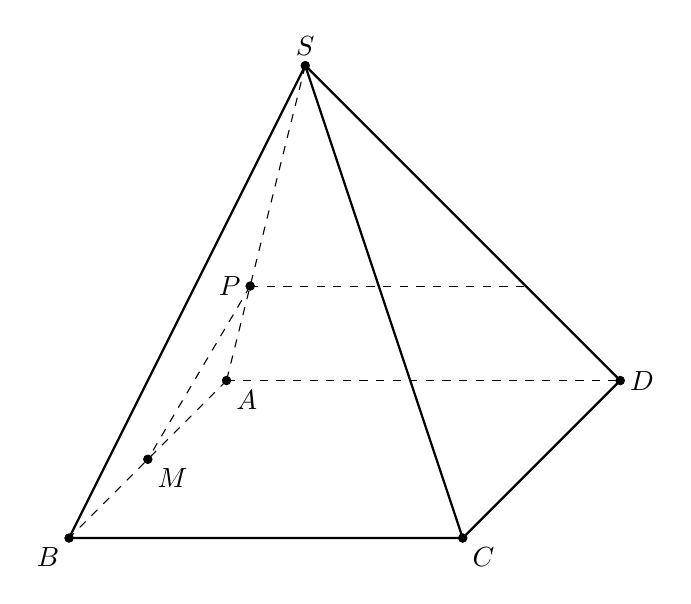
\begin{tikzpicture}
					\coordinate (A) at (0,0);
					\coordinate (B) at (-2,-2);
					\coordinate (C) at (3,-2);
					\coordinate (D) at (5,0);
					\coordinate (S) at (1,4);
					\coordinate (M) at (-1,-1);
					\coordinate (P) at (0.3,1.2);
					\coordinate (P1) at (3.8,1.2);
					\draw [thick] (B) -- (C) -- (D);
					\draw [thick] (S) -- (B);
					\draw [thick] (S) -- (C);
					\draw [thick] (S) -- (D);
					\draw [dashed] (S) -- (A);
					\draw [dashed] (A) -- (B);
					\draw [dashed] (A) -- (D);
					\draw [dashed] (P) -- (P1);
					\draw [dashed] (P) -- (M);
					\filldraw (S) circle(1.5pt) node[above] {$S$};
					\filldraw (A) circle(1.5pt) node[below right] {$A$};
					\filldraw (B) circle(1.5pt) node[below left] {$B$};
					\filldraw (C) circle(1.5pt) node[below right] {$C$};
					\filldraw (D) circle(1.5pt) node[right] {$D$};
					\filldraw (M) circle(1.5pt) node[below right] {$M$};
					\filldraw (P) circle(1.5pt) node[left] {$P$};
				\end{tikzpicture}
		\end{center}
		Ta có: $\heva{&MN \parallel AD\\&MC \subset (PMN)\\&AD \subset (SAD)\\&P \in (PMN) \cap (SAD)}$\\
		Nên giao tuyến của hai mặt phẳng $(SAD)$ và $(PMN)$ là đường thẳng qua $P$ song song với $AD$.
	}
\end{ex}

\begin{ex}%[Câu 10]%[1D5H2-3]
	Trong mẫu số liệu ghép nhóm, tứ phân vị thứ ba $Q_3$ thể hiện:
	\choice
	{Có $25\%$ số giá trị nhỏ hơn $Q_3$}
	{\True Có $75\%$ số giá trị nhỏ hơn $Q_3$}
	{Có $25\%$ số giá trị lớn hơn $Q_3$}
	{Có $75\%$ số giá trị lớn hơn $Q_3$}
	\loigiai{
		Trong mẫu số liệu ghép nhóm, tứ phân vị thứ ba $Q_3$ thể hiện có $75\%$ số giá trị nhỏ hơn $Q_3$.
	}
\end{ex}

\begin{ex}%[Câu 11]%[1D1H2-2]
	Biết rằng $\tan \alpha = 2$. Giá trị biểu thức $\dfrac{\sin \alpha +2 \cos \alpha}{3\sin \alpha - \cos \alpha}\, (\cos \alpha \ne 0)$ là
	\choice
	{$\dfrac{4}{5}$}
	{$1$}
	{$\dfrac{3}{5}$}
	{\True $\dfrac{5}{3}$}
	\loigiai{
		Ta có: $\dfrac{\sin \alpha +2 \cos \alpha}{3\sin \alpha - \cos \alpha} = \dfrac{\dfrac{\sin \alpha}{\cos \alpha} + \dfrac{2 \cos \alpha}{\cos \alpha}}{\dfrac{3\sin \alpha}{\cos \alpha} - \dfrac{\cos \alpha}{\cos \alpha}}=\dfrac{\tan \alpha +2}{3\tan \alpha -1}=\dfrac{2+2}{3 \cdot 2 -1}=\dfrac{4}{5}$.
	}
\end{ex}

\begin{ex}%[Câu 12]%[1D2H2-7]
	Một thửa ruộng bậc thang có thửa thấp nhất (bậc thấp nhất) nằm ở độ cao $900$ mét so với mực nước biển và độ chênh lệch giữa thửa trên và thửa dưới (hai thửa liên tiếp) trung bình là $1{,}5$ mét. Hỏi bậc thứ $19$ của thửa ruộng đó có độ cao là bao nhiêu so với mực nước biển?
	\choice
	{$930$ mét}
	{$928{,}5$ mét}
	{$925{,}5$ mét}
	{\True $927$ mét}
	\loigiai{
		Gọi $u_n$ là chiều cao (mét) so với mực nước biển của thửa ruộng bậc thang ở bậc thứ $n$.\\
		Khi đó, $(u_n)$ là một cấp số cộng với $u_1=900 \text{m}$ và $d=1{,}5 \text{m}$.\\
		Ta có: $u_{19}=u_1+18 \cdot d=900+18 \cdot 1{,}5=927$ mét.\\
		Vậy bậc thứ $19$ của thửa ruộng có độ cao là $927$ mét so với mực nước biển.
	}
\end{ex}
\Closesolutionfile{ans}
\indapan{6}{ans/ans-2-B1-De1-LC}
%-------------------------------------------
\Opensolutionfile{ans}[ans/ans-2-B1-De1-DS]
\cauds
\begin{ex}%[Câu 13]%[1D5V2-3]
	Một hãng xe ô tô thống kê lại số lần gặp sự cố về động cơ của $100$ chiếc xe cùng loại sau $2$ năm sử dụng đầu tiên ở bảng số liệu sau:
	\begin{center}
		\begin{tabular}{|c|c|c|c|c|c|}
			\hline
			Số lần gặp sự cố & $[1;2]$ & $[3;4]$ & $[5;6]$ & $[7;8]$ & $[9;10]$ \\
			\hline
			Số xe & $17$ & $33$ & $25$ & $20$ & $5$ \\
			\hline
		\end{tabular}
	\end{center}
	\choiceTF
	{\True Cỡ mẫu của số liệu là $n=100$}
	{Tứ phân vị thứ nhất của mẫu số liệu ghép nhóm là: $Q_1 \approx 1{,}98$}
	{\True Tứ phân vị thứ hai của mẫu số liệu ghép nhóm là: $Q_2=4{,}5$}
	{\True Tứ phân vị thứ ba của mẫu số liệu ghép nhóm là: $Q_3=6{,}5$}
	\loigiai{
		Gọi $x_1, x_2, x_3, \ldots, x_{100}$ là mẫu số liệu được xếp theo thứ tự không giảm.\\
		Trung vị của của mẫu số liệu là $\dfrac{x_{50}+x_{51}}{2}$ với $x_{50} \in[2{,}5 ; 4{,}5), x_{51} \in[4{,}5 ; 6{,}5)$.
		\begin{itemchoice} 
			\itemch Đúng. Vì cỡ mẫu của mẫu số liệu là $n=100$.
			\itemch Sai. Vì 	xét nửa mẫu số liệu bên trái $x_1, x_2, x_3, \ldots, x_{50}$ có trung vị\\ $\dfrac{x_{25}+x_{26}}{2} \in[2{,}5 ; 4{,}5)$.\\
			Ta có: $n_m=33 ; C=17 ; u_{m+1}=4{,}5 ; u_m=2{,}5$.\\
			Vì vậy, tứ phân vị thứ nhất của mẫu số liệu ghép nhóm là:
			$$
			Q_1=2{,}5+\dfrac{\dfrac{100}{4}-17}{33}(4{,}5-2{,}5)=\dfrac{197}{66} \approx 2{,}98
			$$
			\itemch Đúng. Vì tứ phân vị thứ hai cũng là trung vị của mẫu số liệu ghép nhóm là
			$Q_2=4{,}5$.
			\itemch Đúng. Vì Xét nửa mẫu số liệu bên phải $x_{51}, x_{52}, \ldots, x_{100}$ có trung vị\\
			$\dfrac{x_{75}+x_{76}}{2}$ với $x_{75} \in[4{,}5 ; 6{,}5), x_{76} \in[6{,}5 ; 8{,}5)$ nên tứ phân vị thứ ba của mẫu số liệu ghép nhóm $Q_3=6{,}5$.
		\end{itemchoice}
	}
\end{ex}

\begin{ex}%[Câu 14]%[1H4H4-6]
	Cho hình chóp $S.ABCD$ có đáy là hình bình hành tâm $O$. Gọi $M,\,N$ lần lượt là trung điểm của $SA$ và $SD$. Khi đó:
	\choiceTF
	{$MN \parallel (SBC)$}
	{$(OMN) \parallel (SBC)$}
	{Gọi $E$ là trung điểm đoạn $AB$ và $F$ là một điểm thuộc đoạn $ON$. Khi đó $EF$ cắt với mặt phẳng $(SBC)$}
	{Gọi $G$ là một điểm nằm trên mặt phẳng $(ABCD)$ cách đều $AB$ và $CD$. Khi đó $GN$ cắt $(SAB)$}
	\loigiai{
		Ta xét hình vẽ:
		\begin{center}
			\begin{tikzpicture}
				\coordinate (A) at (0,0);
				\coordinate (S) at (1,4);
				\coordinate (D) at (4,0);
				\coordinate (B) at (-2,-2);
				\coordinate (C) at (2,-2);
				\coordinate (M) at ($(S)!0.5!(A)$);
				\coordinate (N) at ($(S)!0.5!(D)$);
				\coordinate (E) at ($(A)!0.5!(B)$);
				\coordinate (O) at ($(A)!0.5!(C)$);
				\coordinate (F) at ($(N)!0.25!(O)$);
				\coordinate (P1) at ($(A)!0.5!(D)$);
				\coordinate (I) at ($(B)!0.5!(C)$);
				\coordinate (G) at ($(P1)!0.5!(O)$);
				\draw [thick] (S) -- (B);
				\draw [thick] (S) -- (C);
				\draw [thick] (S) -- (D);
				\draw [thick] (B) -- (C) -- (D);
				\draw [dashed] (A) -- (B);
				\draw [dashed] (A) -- (C);
				\draw [dashed] (A) -- (D);
				\draw [dashed] (A) -- (S);
				\draw [dashed] (O) -- (E) -- (M) -- (N) -- cycle;
				\draw [dashed] (E) -- (F);
				\draw [dashed] (M) -- (O);
				\draw [dashed] (I) -- (P1);
				\draw [dashed] (M) -- (G);
				\filldraw (S) circle(1.5pt) node[above] {$S$};
				\filldraw (M) circle(1.5pt) node[above right] {$M$};
				\filldraw (N) circle(1.5pt) node[above right] {$N$};
				\filldraw (F) circle(1.5pt) node[right] {$F$};
				\filldraw (A) circle(1.5pt) node[above right] {$A$};
				\filldraw (D) circle(1.5pt) node[right] {$D$};
				\filldraw (E) circle(1.5pt) node[below right] {$E$};
				\filldraw (O) circle(1.5pt) node[below] {$O$};
				\filldraw (B) circle(1.5pt) node[below left] {$B$};
				\filldraw (C) circle(1.5pt) node[below right] {$C$};
				\filldraw (P1) circle(1.5pt) node[below right] {};
				\filldraw (I) circle(1.5pt) node[below] {$I$};
				\filldraw (G) circle(1.5pt) node[below] {$G$};
			\end{tikzpicture}
		\end{center}
		\begin{itemchoice}
			\itemch Đúng. Vì $MN$ là đường trung bình của tam giác $SAD$ nên $MN \parallel AD$\\
			$\Rightarrow MN \parallel BC \Rightarrow MN \parallel (SBC)$. (1)
			\itemch Đúng. Vì tương tự ta có $O,\,N$ theo thứ tự là trung điểm của $BD,\,SD$ nên $ON$ là đường trung bình của tam giác $SBD \Rightarrow ON \parallel SB \Rightarrow ON \parallel (SBC)$. (2)\\
			Từ (1) và (2) suy ra $(OMN) \parallel (SBC)$.
			\itemch Sai. Vì ta có $OE$ là đường trung bình của tam giác $ABD$ nên $OE \parallel AD \Rightarrow OE \parallel MN$.\\
			Do đó $E \in (OMN)$. Mặt khác $F \in ON$, $ON \subset (OMN) \Rightarrow F \in (OMN)$.\\
			Ta có: $\heva{&EF \subset (OMN)\\&(OMN) \parallel (SBC)} \Rightarrow EF \parallel (SBC)$.
			\itemch Sai. Vì $G$ thuộc mặt phẳng $(ABCD)$ và cách đều $AB,\,CD$ nên $G$ thuộc đường trung bình của hình bình hành $ABCD$ (ứng với hai cạnh $AB,\,CD$).\\
			Gọi $I$ là trung điểm $BC$ thì $I,O,G$ thẳng hàng.\\
			Ta có $OI$ là đường trung bình của $\Delta ABC$ nên $OI \parallel AB \Rightarrow OI \parallel (SAB)$. (3)\\
			Tương tự, ta có $ON \parallel SB \Rightarrow ON \parallel (SAB)$. (4)\\
			Từ (3) và (4) suy ra $(OIN) \parallel (SAB)$ mà $NG \subset (OIN)$ nên $NG \parallel (SAB)$.
		\end{itemchoice}
	}
\end{ex}

\begin{ex}%[Câu 15]%[1D2V1-1]
	Cho dãy số $(u_n)$ có số hạng tổng quát $u_n=1-\dfrac{1}{n}$. Khi đó:
	\choiceTF
	{\True $u_3=\dfrac{2}{3}$}
	{$u_7-u_8=\dfrac{1}{56}$}
	{$u_{n+1}-u_n=-\dfrac{1}{n(n+1)}$}
	{\True Dãy số $(u_n)$ là dãy số tăng}
	\loigiai{
		\begin{itemchoice}
			\itemch Đúng. Vì ta có $u_3=\dfrac{2}{3}$.
			\itemch Sai. Vì $u_7-u_8=-\dfrac{1}{56}$.
			\itemch Sai. Vì ta có $u_{n+1}-u_n=(1-\dfrac{1}{n+1})-(1-\dfrac{1}{n})=\dfrac{1}{n}-\dfrac{1}{n-1}=\dfrac{1}{n(n+1)}>0,\,\forall n \ge 1 $.
			\itemch Đúng. Vì $u_{n+1}-u_n>0 \Rightarrow u_{n+1}>u_n,\,\forall n \in \mathbb{N}^*$. Suy ra dãy số $(u_n)$ là dãy số tăng.
		\end{itemchoice}
	}
\end{ex}

\begin{ex}%[Câu 16]%[1D1V5-3]
	Cho phương trình $\sin \left(2x-\dfrac{\pi}{4}\right)=\sin \left(x+\dfrac{3\pi}{4}\right)$. Các mệnh đề sau đúng hay sai?
	\choiceTF
	{\True Phương trình có nghiệm $\hoac{&x=\pi+k2\pi\\&x=\dfrac{\pi}{6}+k\dfrac{2\pi}{3}}\,(k\in \mathbb{Z})$}
	{\True Trong khoảng $(0;\pi)$ phương trình có 2 nghiệm}
	{Tổng các nghiệm của phương trình trong khoảng $(0;\pi)$ bằng $\dfrac{7\pi}{6}$}
	{\True Trong khoảng $(0;\pi)$ phương trình có nghiệm lớn nhất bằng $\dfrac{5\pi}{6}$}
	\loigiai{
		Ta có:\\
		$\sin \left(2x-\dfrac{\pi}{4}\right)=\sin \left(x+\dfrac{3\pi}{4}\right) \Leftrightarrow \heva{&2x-\dfrac{\pi}{4}=x+\dfrac{3\pi}{4}+k2\pi\\&2x-\dfrac{\pi}{4}=\dfrac{\pi}{4}-x+k2\pi} \Leftrightarrow \heva{&x=\pi+k2\pi\\&x=\dfrac{\pi}{6}+k\dfrac{2\pi}{3}}\,(k \in \mathbb{Z})$.\\
		Vì $x \in (0;\pi)$ nên $x \in \left\{\dfrac{\pi}{6};\dfrac{5\pi}{6}\right\}$.
		Vậy phương trình có 2 nghiệm thuộc khoảng $(0;\pi)$ là $x=\dfrac{\pi}{6};\, x=\dfrac{5\pi}{6}$.
		\begin{itemchoice}
			\itemch Đúng.
			\itemch Đúng.
			\itemch Sai.
			\itemch Đúng.
		\end{itemchoice}
	}
\end{ex}
\Closesolutionfile{ans}
\indapan{2}{ans/ans-2-B1-De1-DS}
%-------------------------------------------
\Opensolutionfile{ans}[ans/ans-2-B1-De1-KQ]
\caukq
\begin{ex}%[Câu 17]%[1D1H2-3]
	Cho hai góc nhọn $a$ và $b$. Biết $\cos a =\dfrac{1}{3}$ và $\cos b=\dfrac{1}{4}$. Tính giá trị của biểu thức $P=(\cos a \cdot \cos b)^2-(\sin a \cdot \sin b)^2$.
	\shortans[0]{$-0{,}8$}
	\loigiai{
		Ta xét:
		\begin{eqnarray*}
			&P&=(\cos a \cdot \cos b)^2-(\sin a \cdot \sin b)^2\\
			& &=(\cos a \cdot \cos b)^2-(1-\cos^2a)(1-\cos^2b)\\
			& &=\left(\dfrac{1}{12}\right)^2-\dfrac{8}{9} \cdot \dfrac{15}{16}\\
			& &=-\dfrac{119}{144} \approx -0{,}8
		\end{eqnarray*}
	}
\end{ex}

\begin{ex}%[Câu 18]%[1D2V2-7]
	Vào đầu mỗi tháng, ông An đều gửi vào ngân hàng số tiền cố định $30$ triệu đồng theo hình thức lãi kép với lãi suất $0{,}6\%$ mỗi tháng. Tính số tiền ông An có được sau tháng sau tháng thứ hai
	\shortans[0]{$60{,}5$}
	\loigiai{
		Số tiền ông An có được:\\
		$\bullet$ Sau tháng thứ nhất là $T_1=30+30 \cdot \dfrac{0{,}6}{100}=30{,}18$ (triệu đồng).\\
		$\bullet$ Sau tháng thứ hai là $T_2=30+30 \left(1+\dfrac{0{,}6}{100}\right)+\left[30+30\left(1+\dfrac{0{,}6}{100}\right)\right]\dfrac{0{,}6}{100} \approx 60{,}54$ (triệu đồng).
	}
\end{ex}

\begin{ex}%[Câu 19]%[1D2V3-8]
	Chu kì bán rã của nguyên tố phóng xạ polonium $210$ là $138$ ngày (nghĩa là sau $138$ ngày khối lượng của nguyên tố đó chỉ còn một nửa). Biết khối lượng còn lại của $20$ gam polonium $210$ sau $7314$
	ngày (khoảng $20$ năm) có dạng $4{,}44 \cdot 10^{-a}$ với $a$ là số nguyên. Tính giá trị của biểu thức $P=a^2$.
	\shortans[0]{225}
	\loigiai{
		Gọi $u_n$ (gam) là khối lượng còn lại của $20$ gam polonium $210$ sau $n$ chu kì bán rã.\\
		Ta có $7\,314$ ngày gồm $53$ chu kì bán rã ($1$ chu kì hết $138$ ngày). Theo đề bài ra, ta cần tính $u_{53}$.\\
		Từ giả thiết suy ra dãy $(u_n)$ là một cấp số nhân với số hạng đầu là $u_1=20$ và công bội $q=0{,}5$.\\
		Suy ra $u_n=20 \cdot(0{,}5)^{n-1}$.\\
		Do đó $u_{53}=20 \cdot(0{,}5)^{52} \approx 4{,}44 \cdot 10^{-15}$. 
	}
\end{ex}

\begin{ex}%[Câu 20]%[1D5H1-4]
	Người ta tiến hành phỏng vấn $50$ người về phim chiếu rạp Lật mặt $6$ của Lý Hải. Người điều tra yêu cầu cho điểm phim theo thang điểm $100$. Kết quả được trình bày trong bảng phân bố tần số ghép lớp sau đây:
	\begin{center}
		\begin{tabular}{|c|l|l|l|l|l|}
		\hline Số điểm & {$[50 ; 60)$} & {$[60 ; 70)$} & {$[70 ; 80)$} & {$[80 ; 90)$} & {$[90 ; 100)$} \\
		\hline Số người & $4$ & $7$ & $9$ & $18$ & $12$ \\
		\hline
	\end{tabular}
	\end{center}
	Hãy ước lượng số trung bình và mốt của mẫu số liệu ghép nhóm ở trên.
	\shortans[0]{2}
	\loigiai{
		\begin{center}
			\begin{tabular}{|l|l|l|l|l|l|}
			\hline Số điềm & {$[50 ; 60)$} & {$[60 ; 70)$} & {$[70 ; 80)$} & {$[80 ; 90)$} & {$[90 ; 100)$} \\
			\hline \begin{tabular}{l} 
				Giá trị đại \\
				diện
			\end{tabular} & $55$ & $65$ & $75$ & $85$ & $95$ \\
			\hline Số người & $4$ & $7$ & $9$ & $18$ & $12$ \\
			\hline
		\end{tabular}
		\end{center}
		\begin{itemize}
			\item Điểm trung bình đánh giá phim Lật Mặt $6$ bằng:
			$$
			\dfrac{55 \cdot 4+65 \cdot 7+75 \cdot 9+85 \cdot 18+95 \cdot 12}{50}=80{,}4
			$$
			\item Nhóm chứa mốt của mẫu số liệu trên là $[80 ; 90)$.\\
			Do đó: $u_m=80 ; n_{m-1}=9 ; n_{m+1}=12 ; u_{m+1}-u_m=90-80=10$.
		\end{itemize}
		Mốt của mẫu số liệu ghép nhóm là: $M_o=80+\dfrac{18-9}{(18-9)+(18-12)} \cdot 10=80{,}6$.
	}
\end{ex}

\begin{ex}%[Câu 21]%[1D3H3-3]
	Tìm giá trị của $m$ để hàm số $f(x)=\heva{&\dfrac{x^2-x-2}{x-2},\, \text{nếu } x \ne 2 \\&m+1, \, \text{nếu } x=2}$ liên tục tại điểm $x_0=2$.
	\shortans[0]{2}
	\loigiai{
		Ta có: $f(2)=m+1$;
		$$
		\lim _{x \rightarrow 2} f(x)=\lim _{x \rightarrow 2} \dfrac{x^2-x-2}{x-2}=\lim _{x \rightarrow 2} \dfrac{(x-2)(x+1)}{x-2}=\lim _{x \rightarrow 2}(x+1)=3.
		$$
		Hàm số liên tục tại $x_0=2$ khi và chỉ khi $ \lim\limits_{x\to a} f(x)=f(2) \Leftrightarrow m+1=3 \Leftrightarrow m=2$.
	}
\end{ex}

\begin{ex}%[Câu 22]%[1D1C4-6]
	Tìm tổng giá trị lớn nhất và giá trị nhỏ nhất của hàm số $y=\dfrac{2\sin x+3\cos x+1}{\sin x-\cos x+2}$
	\shortans[0]{3}
	\loigiai{
		Lý thuyết: $a\sin x +b \cos x =c$. Phương trình có nghiệm khi $a^2+b^2 \ge c^2$.\\
		Ta có: $y=\dfrac{2 \sin x+3 \cos x+1}{\sin x-\cos x+2} \Leftrightarrow(y-2) \sin x-(y+3) \cos x=1-2 y$.\\
		Điều kiện để tồn tại cặp số $(x ; y)$ là\\ $(y-2)^2+(y+3)^2 \geq(1-2 y)^2$ $\Leftrightarrow-2 y^2+6 y+12 \geq 0 \Leftrightarrow \dfrac{3-\sqrt{33}}{2} \leq y \leq \dfrac{3+\sqrt{33}}{2}$.\\
		Tổng giá trị lớn nhất và giá trị nhỏ nhất của hàm số: $\dfrac{3-\sqrt{33}}{2}+\dfrac{3+\sqrt{33}}{2}=3$.
	}
\end{ex}
\Closesolutionfile{ans}
\indapan{6}{ans/ans-2-B1-De1-KQ}